\documentclass[11pt,a4paper]{article}

\usepackage[utf8]{inputenc}
\usepackage[T1]{fontenc}
\usepackage[english]{babel}
\usepackage[a4paper,margin=2.4cm]{geometry}

\usepackage{amsmath, amssymb, amsthm}
\usepackage{mathtools}
\usepackage{stmaryrd}
\usepackage{booktabs}
\usepackage{tabularx}
\usepackage{array}
\usepackage{caption}
\usepackage{subcaption}
\usepackage{float}
\usepackage{enumitem}
\usepackage{microtype}
\usepackage{xcolor}
\usepackage{listings}
\usepackage{fancyhdr}
\usepackage{titlesec}
\usepackage{graphicx}
\usepackage{tikz}
\usetikzlibrary{positioning, arrows.meta, fit, backgrounds, calc, shapes.geometric}
\usepackage[hidelinks]{hyperref}

%  ---  Palette shared with the companion reports  ---
\definecolor{ink}{RGB}{26,30,36}
\definecolor{slate}{RGB}{92,101,112}
\definecolor{mist}{RGB}{233,235,238}
\definecolor{rulegrey}{RGB}{188,194,201}
\definecolor{steel}{RGB}{47,72,102}
\definecolor{steellight}{RGB}{124,146,172}
\definecolor{signal}{RGB}{160,32,45}
\definecolor{southc}{RGB}{51,115,204}
\definecolor{northc}{RGB}{230,128,38}
\definecolor{knows}{RGB}{26,140,70}

\hypersetup{
    colorlinks=true,
    linkcolor=steel,
    citecolor=steel,
    urlcolor=steel,
    pdftitle={The Lookout Board},
    pdfauthor={Haniel Ulises},
}

\color{ink}

\setlength{\headheight}{22pt}
\pagestyle{fancy}
\fancyhf{}
\fancyhead[L]{\small\textcolor{slate}{\itshape The Lookout Board}}
\fancyhead[R]{\small\textcolor{slate}{\thepage}}
\renewcommand{\headrulewidth}{0.4pt}
\renewcommand{\headrule}{\hbox to\headwidth{\color{rulegrey}\leaders\hrule height \headrulewidth\hfill}}

\titleformat{\section}{\normalfont\large\bfseries\color{ink}}{\thesection}{0.7em}{}
\titleformat{\subsection}{\normalfont\normalsize\bfseries\color{ink}}{\thesubsection}{0.7em}{}
\titleformat{\paragraph}[runin]{\normalfont\bfseries\color{slate}}{}{0em}{}[.]

\captionsetup{font=small, labelfont={bf,color=slate}, textfont=footnotesize}

\theoremstyle{definition}
\newtheorem{definition}{Definition}
\newtheorem{proposition}{Proposition}
\newtheorem{lemma}{Lemma}
\newtheorem{corollary}{Corollary}
\newtheorem{fact}{Fact}
\newtheorem{remark}{Remark}

\lstdefinestyle{sys}{
    backgroundcolor=\color{mist},
    basicstyle=\ttfamily\scriptsize\color{ink},
    keywordstyle=\color{steel}\bfseries,
    commentstyle=\color{slate}\itshape,
    stringstyle=\color{slate},
    morecomment=[l]{;},
    morekeywords={:types,:predicates,:objects,:agents,:goal,:init,:event,:action,:action-type,:observability-conditions,:precondition,:effects,:events,:relations,:designated,:conditions,:observability-types},
    frame=single,
    rulecolor=\color{rulegrey},
    framesep=5pt,
    xleftmargin=6pt,
    xrightmargin=0pt,
    breaklines=true,
    showstringspaces=false,
    columns=fullflexible,
    captionpos=b,
}
\lstset{style=sys}

%  ---  Notation  ---
\newcommand{\Ag}{\mathcal{A}}
\newcommand{\Mod}{\mathcal{M}}
\newcommand{\Ev}{\mathcal{E}}
\newcommand{\prd}{\otimes}
\newcommand{\Kop}[1]{K_{#1}}
\newcommand{\Eop}[1]{E_{#1}}
\newcommand{\Cop}[1]{C_{#1}}
\newcommand{\Kw}[1]{\mathit{Kw}_{#1}}
\newcommand{\code}[1]{\texttt{\small #1}}
\newcommand{\ag}[1]{\mathit{#1}}
\newcommand{\job}{\mathit{job}}
\newcommand{\pre}{\mathit{pre}}
\newcommand{\post}{\mathit{post}}
\newcommand{\dist}{\mathrm{dist}}
\newcommand{\depth}{\mathrm{depth}}

\newcommand{\cl}[1]{\mathit{clear\text{-}#1}}
\newcommand{\bz}{\mathit{blocked\text{-}z}}
\newcommand{\at}[1]{\mathit{at\text{-}#1}}
\newcommand{\act}[1]{\textsf{#1}}

\begin{document}

\begin{titlepage}
\centering
\vspace*{2.4cm}
{\color{rulegrey}\rule{\textwidth}{0.8pt}}\\[0.9cm]
{\LARGE\bfseries The Lookout Board\par}
\vspace{0.5cm}
{\large\color{slate} Information Gathering an Epistemic Planner Chooses\\
and No Classical Planner Can\par}
\vspace{0.7cm}
{\color{rulegrey}\rule{\textwidth}{0.8pt}}\\[1.4cm]

{\large Haniel Ulises\par}
\vspace{0.3cm}
{\color{slate} Epistemic Robotics}\\
\vspace{0.15cm}
{\color{slate}13 October 2026}

\vfill
{\color{slate}\small
A robot must know whether a zone is blocked. It can see the zone through four
windows, one from each of four lookouts, but a screen closes every window
except one, and which one is open is not known. A status board beside the
robot's start shows it: slot $k$ is lit exactly when the view from lookout $k$
is clear. Nothing in the goal mentions the board. We prove that the domain has
no conformant plan, that the policy of depth six Aletheia returns reads the
board, goes to the lookout it shows lit and goes to the last lookout unread
when three slots are dark, and that no classical planner reads the board: not
a planner over the classical model, in which reading achieves nothing a goal
needs; not one over a knowledge-level compilation under any determinization of
its outcomes, since the board is a detour; and not hindsight optimisation,
under which sensing has no value. On the roadmap of the hall the policy drives
8.47\,m on average over the eight worlds and 12.15\,m at worst; replanning from
the nearest lookout drives 13.91\,m and 24.66\,m; the conformant tour 24.66\,m
always. In Gazebo, 32 paired seeds under each formulation measure it:
every run of every formulation ended knowing the zone, backed by the map; the
policy read the board in 32 of 32 runs and the classical ones in
none; mean mission time was 48.0\,s for the policy, 77.4\,s for
replanning and 134.0\,s for the tour, and the policy's worst
66.6\,s against 137.1\,s and 137.4\,s.}
\vspace{1.2cm}
\end{titlepage}

\tableofcontents
\newpage

%  ======================================================================
\section{Scope}

The comparison of epistemic and classical planning is usually made where the
classical planner is handicapped: given a sequence to commit to, or denied the
observations the epistemic planner gets. This report makes it where the
classical side is at its strongest. The classical planner is POPF~\cite{popf2010}, with every
action of the epistemic domain in its model, the duration of every drive taken
from the roadmap the robot drives, and looks that end as soon as the map
decides the zone or shows the window screened; in one formulation it replans
after every look from where the robot stands, with the lookouts already found
screened removed. What it is not given is a model of what the robot will know.

The scenario is built so that this is the one thing that matters. Reading the
board achieves nothing the goal asks for; it only changes what the robot knows,
and through that, where it should go. An epistemic planner sees the change,
because its states are what the robot knows. A classical planner does not, and
the propositions of Section~\ref{sec:classical} show that no determinization
of the sensing outcomes, and no sampling of worlds, makes it see it.

%  ======================================================================
\section{The hall}

\begin{figure}[H]
\centering
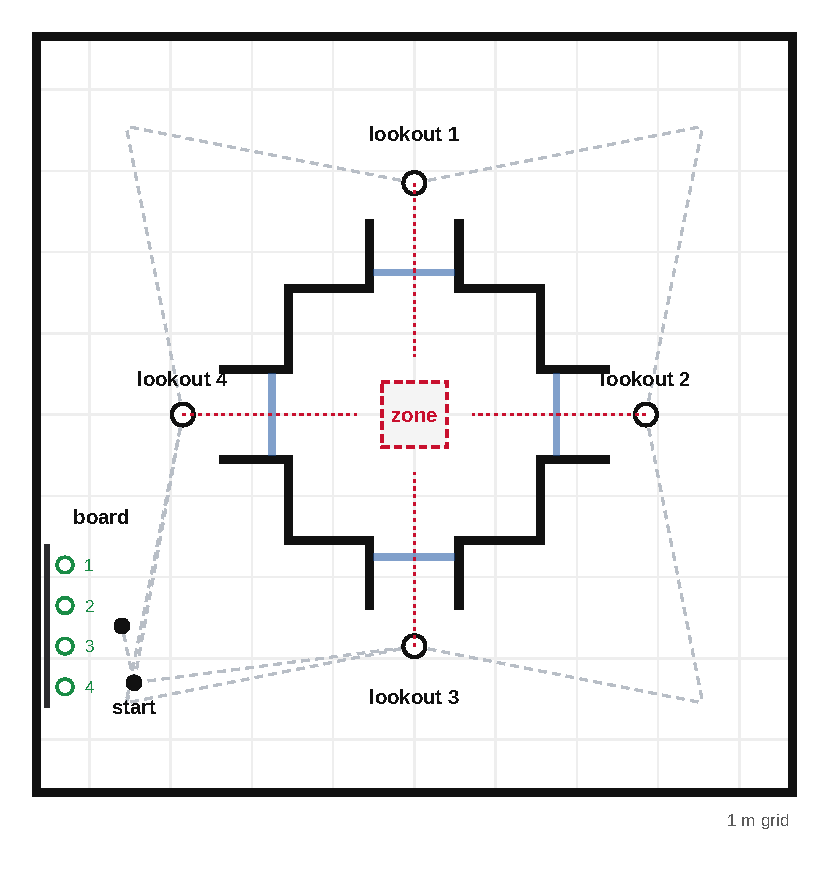
\includegraphics[width=0.62\textwidth]{figures/lookout_board_floor.pdf}
\caption{The hall, 9.2 by 9.2\,m. The zone, a 0.8\,m square, stands in the
middle of a walled room with a window in each wall; each window opens onto an
embrasure, a channel 0.8\,m deep between two side walls, and lookout $k$
stands in front of embrasure $k$. The blue bars are where a screen stands; all
but one do. The board is a panel against the west wall with four slots before
it, and the robot reads it from 0.7\,m off its start. Dashed: the roadmap the
drive node plans over.}
\label{fig:hall}
\end{figure}

\noindent
The embrasures make a view of the zone a property of standing at a lookout: a
robot passing along the corridor sees the side walls of an embrasure and
nothing of the room. A screen, when it stands, closes its window from inside
the embrasure, so a robot at a screened lookout sees the screen and not the
zone. The robot is a TurtleBot3 Burger with its laser's range set to 8\,m (the
LDS-01 reaches 3.5\,m, too short to see across the room), mapping with
slam\_toolbox. Eight worlds, one per open lookout and per zone, blocked by a
crate or clear; seed $s$ takes world $(s-1) \bmod 8$ and perturbs the start by
up to 0.1\,m and $10^\circ$.

Before any simulator run, \code{tools/check\_views.py} casts the laser over a
rasterised floor in every world and checks that each observation means what the
domain says: from lookout $k$ the zone is decided exactly when the view from
$k$ is clear, and the window reads blocked exactly when it is not; at the board
the lit slot reads blocked and the other three clear; and no route the robot
drives between two places decides the zone in passing.

%  ======================================================================
\section{The domain}

One agent, $r1$. Atoms: $\bz$; $\cl{1}, \ldots, \cl{4}$, the view from lookout
$k$ is clear; and where the robot stands, $\at{board}$ and $\at{l_k}$. Actions,
as event models~\cite{bms1998}, planned over as in~\cite{ba2011}:

\begin{center}
\small
\begin{tabularx}{\textwidth}{@{}l l X X@{}}
\toprule
action & kind & precondition & events \\
\midrule
\act{goto-board}, \act{goto-l$k$} & public ontic & not already there & there, and nowhere else \\
\act{read-$k$} & sensing & $\at{board}$ & lit where $\cl{k}$, dark where $\neg\cl{k}$ \\
\act{check-$k$} & sensing & $\at{l_k}$ & clear where $\cl{k}$, screened where $\neg\cl{k}$ \\
\act{look-$k$} & sensing & $\at{l_k} \wedge K_{r1}\cl{k}$ & blocked where $\bz$, free where $\neg\bz$ \\
\bottomrule
\end{tabularx}
\end{center}

\noindent
The sensing actions are semi-private. The initial model has eight worlds, all
designated, with $r1$'s relation universal and the frame S5: exactly one of
$\cl{1}, \ldots, \cl{4}$ holds, which is therefore common knowledge, and $\bz$
either way. The goal is $\Kw{r1}\,\bz$. Nothing in it, and nothing in any
precondition, mentions the board.

The sensing events carry no condition that the robot not yet know the answer,
which such domains usually have to keep a planner from looking twice. On the
robot every slot of the board resolves at once, and the epistemic state applies
each observation as soon as its event is applicable; with that condition, the
dark slots applied first would make the lit one known by elimination and its
read inapplicable, and the executor would refuse the very action the policy
runs next. Without it, reading what is already known changes nothing, and the
planner still never does it.

%  ======================================================================
\section{The policy}

\begin{proposition}[No conformant plan]
No sequence of the domain's actions is applicable in all eight worlds and
leaves $\Kw{r1}\,\bz$ true in all of them.
\end{proposition}

\begin{proof}
Only the looks' events differ on $\bz$, so such a sequence contains a look;
take the first, \act{look-$k$}. Its precondition must hold in the state reached
from every world, in particular from one where $\neg\cl{k}$, and no action
changes $\cl{k}$; in an S5 model $K_{r1}\cl{k}$ implies $\cl{k}$, so it fails
there.
\end{proof}

\begin{proposition}[The policy]
The policy
\[
\act{goto-board};\ \act{read-1};\
\begin{cases}
\text{lit}: & \act{goto-l1};\ \act{look-1}\\
\text{dark}: & \act{read-2};\
\begin{cases}
\text{lit}: & \act{goto-l2};\ \act{look-2}\\
\text{dark}: & \act{read-3};\
\begin{cases}
\text{lit}: & \act{goto-l3};\ \act{look-3}\\
\text{dark}: & \act{goto-l4};\ \act{look-4}
\end{cases}
\end{cases}
\end{cases}
\]
is applicable in all eight worlds, reaches $\Kw{r1}\,\bz$ in all of them, drives
to exactly one lookout, the open one, and has depth 6.
\end{proposition}

\begin{proof}
At the board, \act{read-$k$} lit leaves designated the two worlds where $\cl{k}$,
in which $K_{r1}\cl{k}$ holds, so after \act{goto-l$k$} \act{look-$k$} is
applicable. If slots 1, 2 and 3 are dark, the designated worlds are the two
where $\neg\cl{1} \wedge \neg\cl{2} \wedge \neg\cl{3}$, and since exactly one
view is clear, $\cl{4}$ holds in both: $K_{r1}\cl{4}$ without reading slot 4.
Each look's events split the designated worlds by $\bz$. The longest branch is
\act{goto-board}, three reads, a drive and a look.
\end{proof}

\noindent
Aletheia returns exactly this policy, by AO* in 20\,050 expansions,
and its validator checks all eight leaves. The policy that checks the lookouts
in turn, the only alternative the domain offers, has depth 8. Aletheia
minimises depth, the number of actions on the longest branch, and not distance;
on this hall the two agree, and Section~\ref{sec:cost} gives the distances.

%  ======================================================================
\section{No classical planner reads the board}
\label{sec:classical}

\begin{proposition}[The classical model]
In the classical model the robot executes, \act{read\_slot} achieves nothing
any precondition or goal uses. So no plan that is minimal under removal of
actions contains it, and POPF never returned one.
\end{proposition}

\begin{proof}
The effect of \act{read\_slot}, \textit{read}, occurs in no precondition and
in neither goal, the zone known or every lookout looked from, and the action
deletes nothing. Removing every occurrence from a valid plan leaves it valid
and shorter. Over the batch, POPF returned 80 plans to the replanner,
and none contained \act{read\_slot}.
\end{proof}

\noindent
The classical model is the strongest one a classical planner can be given only
if a model of knowledge would not help it. It would, as far as the
preconditions go: the usual compilation of knowledge into a classical
problem~\cite{pg2009} has fluents for what is known, and a look needing
$K\,\cl{k}$ becomes a look needing a fluent \textit{known-clear-$k$}, which
\act{read-$k$} lit and \act{check-$k$} clear achieve. What such a planner
still has to do is choose an outcome for each sensing action, since it plans
sequences, and the two ways of doing that do not change the result.

\begin{proposition}[Determinization]
Under any determinization that lets the planner choose each sensing action's
outcome, as FF-Replan's all-outcomes determinization does~\cite{yfg2007}, the
cheapest plan does not visit the board.
\end{proposition}

\begin{proof}
The board is a spur off the start, so $d(\mathit{board}, x) = d(s, \mathit{board})
+ d(s, x)$ for every place $x$. A plan through the board reaches some lookout
$k$ known clear at cost at least $2\,d(s,\mathit{board}) + d(s, l_k)$ plus a read;
the plan that drives to $l_k$, checks the view and chooses the outcome clear
reaches the same state at $d(s, l_k)$ plus a check, which is cheaper since the
two sensing actions take the same time. After a failure the robot is at a
lookout $l$, and by the triangle inequality $d(l, \mathit{board}) +
d(\mathit{board}, l_k) \geq d(l, l_k) + 2\,d(s, \mathit{board})$.
\end{proof}

\begin{proposition}[Hindsight]
Hindsight optimisation~\cite{yfgk2008}, which samples worlds and values each action by the
cost of the optimal plan in each sample as though the sample were known, gives
every sensing action a value no better than not sensing, and so never reads the
board.
\end{proposition}

\begin{proof}
In a sampled world the optimal continuation is a plan in a fully known world,
in which a sensing action changes nothing and costs time. Each action's value
is a mean of such continuations, and reading only adds its own cost to each.
\end{proof}

\noindent
A planner that does choose to read the board must value what the robot will
know after reading it, in each of the worlds it cannot yet tell apart. That is
a planner over states of knowledge, which is what an epistemic planner is.

%  ======================================================================
\section{What it costs to drive}
\label{sec:cost}

The roadmap's shortest routes, in metres, give each formulation's drive in
each world exactly, before a robot moves.

\begin{table}[H]
\centering
\small
\begin{tabular}{@{}lrrrrrr@{}}
\toprule
open lookout & 1 & 2 & 3 & 4 & mean & worst \\
\midrule
policy: start, board, $l_c$ & 12.03 & 12.15 & 4.92 & 4.79 & \textbf{8.47} & \textbf{12.15} \\
replanning: $l_4, l_3, l_2, l_1$ until open & 24.66 & 17.42 & 10.18 & 3.35 & 13.91 & 24.66 \\
conformant: the tour $l_4, l_3, l_2, l_1$ & 24.66 & 24.66 & 24.66 & 24.66 & 24.66 & 24.66 \\
\bottomrule
\end{tabular}
\caption{Route lengths over the roadmap.}
\end{table}

\noindent
The replanner's order is POPF's: the nearest lookout by route time, lookout 4,
then from each failure the nearest not yet tried. The conformant tour is the
shortest of the twenty-four orders, lookout 4, 3, 2, 1; POPF's own tour for the
same goal was longer, 193\,s of driving against 155\,s, and the baseline is
given the shorter. The policy pays 1.44\,m for the board in every world and
saves a tour of the room in three of four.

%  ======================================================================
\section{Planning as the lookouts grow}

\begin{table}[H]
\centering
\small
\begin{tabular}{@{}rrrlrlrr@{}}
\toprule
$n$ & worlds & actions & strategy & depth (board / in turn) & first move & expansions & seconds \\
\midrule
2 & 4 & 9 & AO$^*$ & 4 (4 / 4) & lookout 1 & 58 & 0.00 \\
3 & 6 & 13 & AO$^*$ & 5 (5 / 6) & the board & 1497 & 0.01 \\
4 & 8 & 17 & AO$^*$ & 6 (6 / 8) & the board & 20050 & 0.14 \\
5 & 10 & 21 & AO$^*$ & 7 (7 / 10) & the board & 318380 & 2.48 \\
6 & 12 & 25 & replan & 12 (8 / 12) & lookout 1 & 17 & 5.00 \\
6 & 12 & 25 & AO$^*$ alone & 8 (8 / 12) & the board & 5832186 & 46.97 \\
7 & 14 & 29 & replan & 14 (9 / 14) & lookout 1 & 20 & 5.00 \\
7 & 14 & 29 & \multicolumn{4}{l}{AO$^*$ alone: no policy within the budget} & 900 \\
8 & 16 & 33 & replan & 16 (10 / 16) & lookout 1 & 23 & 5.00 \\
\bottomrule
\end{tabular}
\caption{Aletheia on the domain with $n$ lookouts, exactly one of them open:
the grounded size, the strategy its selection policy settled on, the
policy's depth against $n+2$ for reading the board and $2n$ for checking the
lookouts in turn, and the wall-clock time.}
\end{table}

With three to five lookouts, AO$^*$, which Aletheia's selection policy picks, returns the policy that reads the board, of depth $n + 2$, against $2n$ for checking the lookouts in turn; with two the depths tie and it checks. Its search grows by an order of magnitude per lookout. From six lookouts the selection policy gives AO$^*$ a few seconds and then falls back on replanning, which determinizes the sensing outcomes and returns the policy that checks the lookouts in turn, of depth $2n$: the classical planner's policy, and it does not read the board, as a determinizing planner never does. Given the whole budget alone, AO$^*$ finds the board-first policy for six lookouts in 47\,s and 5.8 million expansions, and for seven does not finish in 900\,s. Reading the board is what a planner over states of knowledge finds; finding it is what such a planner pays for.

%  ======================================================================
\section{32 seeds in Gazebo}

Each seed fixes the world and the start, and is run under all three
formulations side by side, so the comparison is paired. Times are simulated
seconds from the order to the end of the mission; distances come from the
robot's odometry, which the simulator reports in the world frame.

\begin{table}[H]
\centering
\small
\begin{tabular}{@{}lrrrrrr@{}}
\toprule
& backed & read the board & mean time & worst time & mean driven & worst driven \\
\midrule
epistemic policy & 32/32 & 32/32 & 48.0\,s & 66.6\,s & 8.1\,m & 12.0\,m \\
classical replanning & 32/32 & 0/32 & 77.4\,s & 137.1\,s & 13.9\,m & 24.8\,m \\
conformant tour & 32/32 & 0/32 & 134.0\,s & 137.4\,s & 24.6\,m & 24.9\,m \\
\bottomrule
\end{tabular}
\caption{The batch, per formulation.}
\end{table}

\begin{table}[H]
\centering
\small
\begin{tabular}{@{}lccc@{}}
\toprule
world & epistemic & replanning & conformant \\
\midrule
lookout 1, zone clear & 64.5\,s, 11.4\,m & 136.4\,s, 24.6\,m & 135.1\,s, 24.6\,m \\
lookout 1, zone blocked & 63.9\,s, 11.4\,m & 136.3\,s, 24.6\,m & 134.8\,s, 24.7\,m \\
lookout 2, zone clear & 66.0\,s, 11.8\,m & 97.1\,s, 17.4\,m & 134.8\,s, 24.7\,m \\
lookout 2, zone blocked & 65.2\,s, 11.7\,m & 97.3\,s, 17.5\,m & 134.6\,s, 24.7\,m \\
lookout 3, zone clear & 32.2\,s, 4.7\,m & 57.3\,s, 10.2\,m & 135.3\,s, 24.6\,m \\
lookout 3, zone blocked & 30.9\,s, 4.7\,m & 56.5\,s, 10.1\,m & 133.0\,s, 24.6\,m \\
lookout 4, zone clear & 31.1\,s, 4.3\,m & 19.3\,s, 3.5\,m & 132.6\,s, 24.7\,m \\
lookout 4, zone blocked & 30.8\,s, 4.3\,m & 18.4\,s, 3.4\,m & 131.0\,s, 24.6\,m \\
\bottomrule
\end{tabular}
\caption{By world: median time and distance; each world met 4 times.}
\end{table}

Every run of every formulation ended knowing the zone, and the map backed it in all 96. The policy read the board in all 32 of its runs, and neither classical formulation read it once. Paired by seed against replanning, the policy was faster in 24 seeds and slower in 8 (exact sign test, $p = 0.007$); the Hodges--Lehmann estimate of what it saves is 29.6\,s and 5.6\,m. It was slower only in the worlds where the open lookout is the replanner's first, by at most 12.7\,s, the price of the board. Against the conformant tour it was faster in 32 of 32 seeds, by 86.0\,s.

%  ======================================================================
\section{The film}

Four takes, recorded one at a time with the launch unchanged and headless: a Gazebo client and RViz on a virtual display, the world held paused until both had drawn, and the Gazebo camera cut on the executor's own actions. Seed 1, where the open view is lookout 1's, the farthest from the start and the replanner's last, under all three formulations; and the policy on seed 8, where lookout 4 is open and the zone blocked, and the policy goes to lookout 4 with slot 4 unread. The film ends with seed 1's policy and replanner side by side by simulated time since the order.

\begin{figure}[H]
\centering
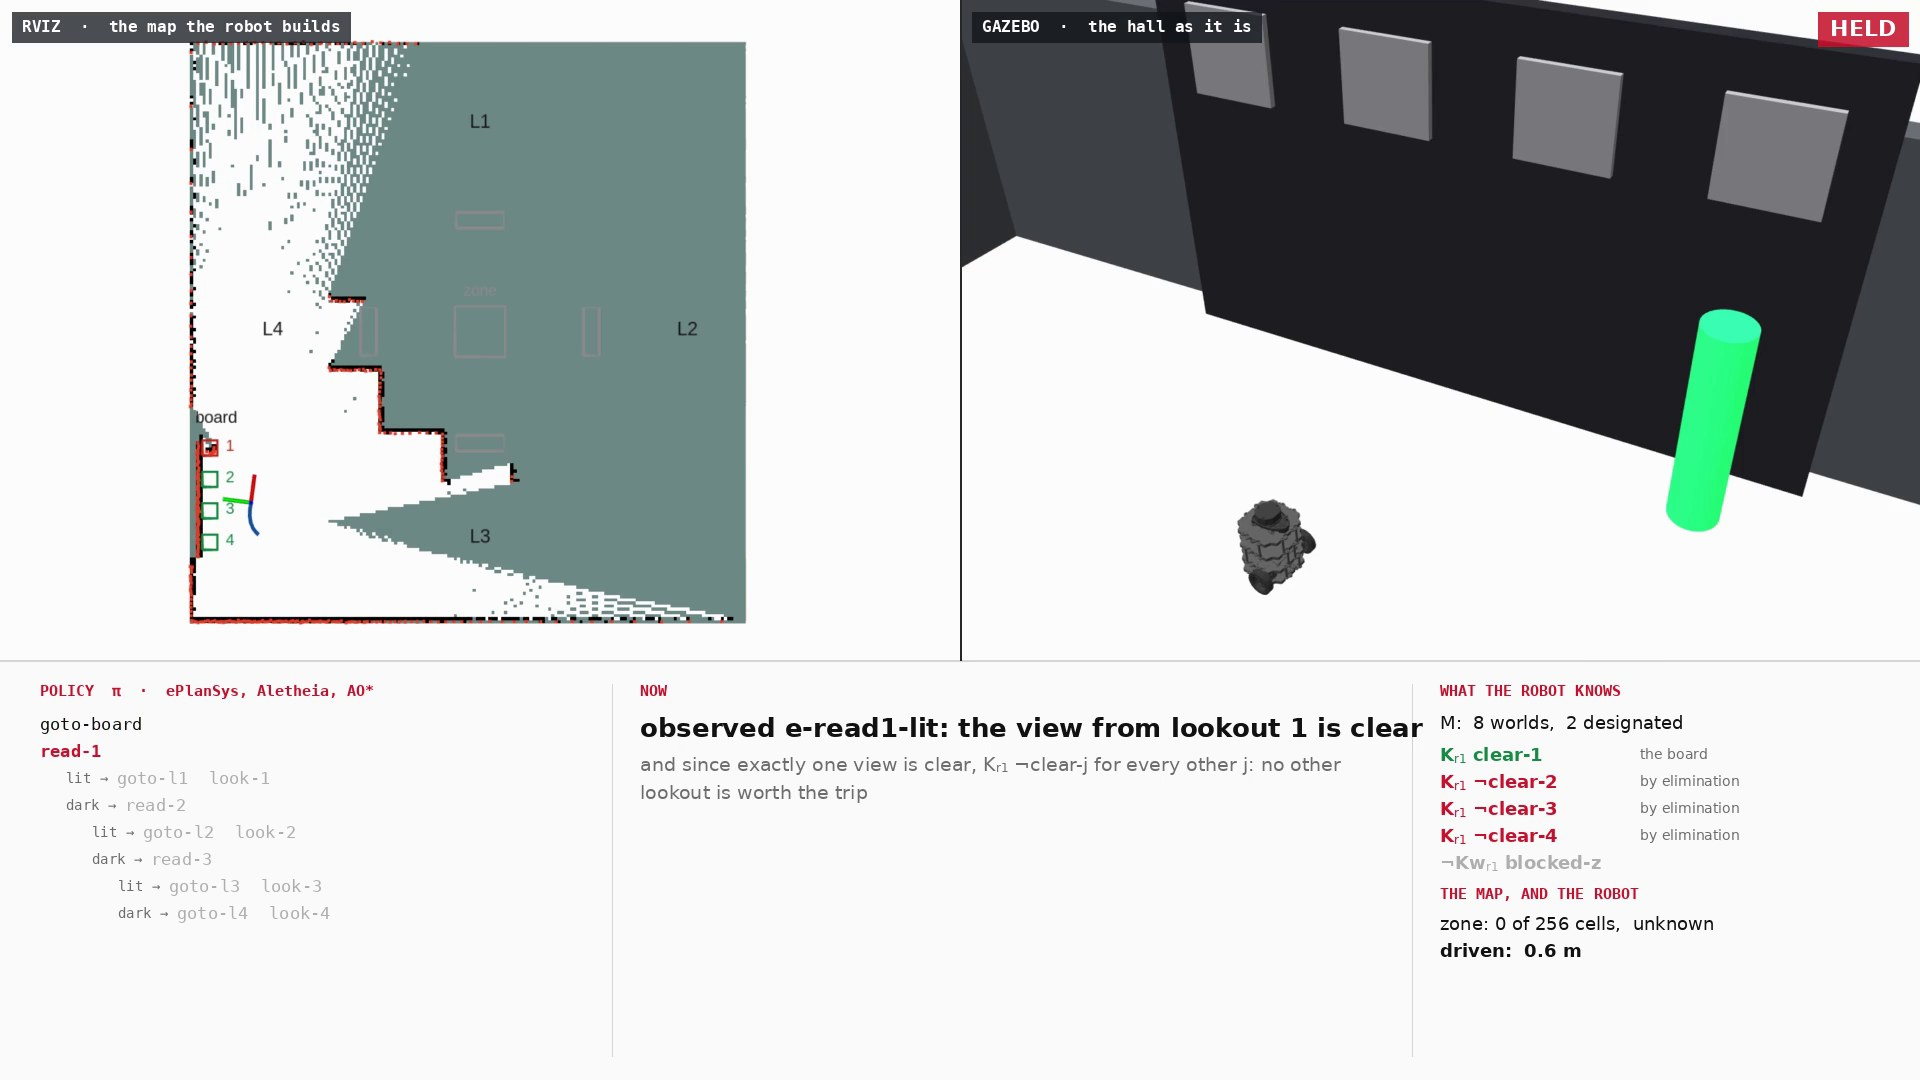
\includegraphics[width=\textwidth]{figures/lookout_board_frame.jpg}
\caption{The film at the board on seed 1, held. Left, RViz: the map, with the
board's slots outlined in the colour the map gives them, slot 1 red (a post
stands in it, so it is lit) and the others green, and the robot's trail from
the start. Right, Gazebo: the robot before the board and slot 1's post. Under
both: the policy with \act{read-1} running, the observation, and what the
robot knows: $K_{r1}\,\cl{1}$ from the board, and $K_{r1}\neg\cl{j}$ for the
other three by elimination.}
\end{figure}

%  ======================================================================
\section{Found on the way}

\paragraph{The guard on sensing}
The first domain had each sensing event require that the robot not yet know
its answer. It planned the same policy, but on the robot it could not run, as
the domain section explains, and the condition was removed. The planner's
policy did not change.

\paragraph{POPF and a negative precondition}
With the look written as requiring \textit{(not (screened ?l))}, POPF dumped
core while building its lookup tables. The classical domain writes it
positively, \textit{open\_view}, which the problem asserts for every lookout not
yet found screened.

\paragraph{A shared scratch file}
PlanSys2's domain expert checks the domain with a POPF instance of its own,
whose scratch directory defaults to \code{/tmp}. Runs started side by side
read each other's half-written \code{check\_domain.pddl}, and two runs of
the batch failed to start with ``PDDL syntax error''. The launch now gives the
domain expert the run's own directory, the batch starts each run a few seconds
apart, and the failed runs were run again; their first attempts are kept.

\paragraph{A parameter outlived}
Both action nodes first iterated directly over the string array of a
parameter, a reference into a temporary that the loop outlived, and aborted with
\code{std::length\_error} at start. They copy the list first.

%  ======================================================================
\section{What this does not show}

\begin{itemize}[leftmargin=1.4em]
\item Cost-aware epistemic planning. Aletheia minimises the policy's depth.
Were the board far away, a policy of least depth could still read it and drive
further than checking the nearest lookout; this hall does not test that.
\item A planner over beliefs that is not epistemic in name. A POMDP solver, or
a contingent planner over belief states, values the board for the same reason
the epistemic planner does; the comparison here is with classical planning.
\item A hand-written rule. ``Read the board first'' would do as well here and
needs no planner; the point is that the epistemic planner finds it from the
domain, and would not on a hall where the board told it nothing.
\item More than one robot, and sensing that can be wrong. The laser's noise is
0.01\,m and every region decided correctly in every run.
\end{itemize}

%  ======================================================================
\begin{thebibliography}{9}
\bibitem{bms1998} A.~Baltag, L.~S. Moss and S.~Solecki.
The logic of public announcements, common knowledge, and private suspicions.
\emph{Proceedings of TARK VII}, 43--56, 1998.
\bibitem{ba2011} T.~Bolander and M.~B. Andersen.
Epistemic planning for single- and multi-agent systems.
\emph{Journal of Applied Non-Classical Logics} 21(1):9--34, 2011.
\bibitem{pg2009} H.~Palacios and H.~Geffner.
Compiling uncertainty away in conformant planning problems with bounded width.
\emph{Journal of Artificial Intelligence Research} 35:623--675, 2009.
\bibitem{yfg2007} S.~Yoon, A.~Fern and R.~Givan.
FF-Replan: a baseline for probabilistic planning.
\emph{Proceedings of ICAPS}, 352--359, 2007.
\bibitem{yfgk2008} S.~Yoon, A.~Fern, R.~Givan and S.~Kambhampati.
Probabilistic planning via determinization in hindsight.
\emph{Proceedings of AAAI}, 1010--1016, 2008.
\bibitem{popf2010} A.~J. Coles, A.~I. Coles, M.~Fox and D.~Long.
Forward-chaining partial-order planning.
\emph{Proceedings of ICAPS}, 42--49, 2010.
\end{thebibliography}

\end{document}
